\section{Key Findings}

\begin{figure}
    \centering
    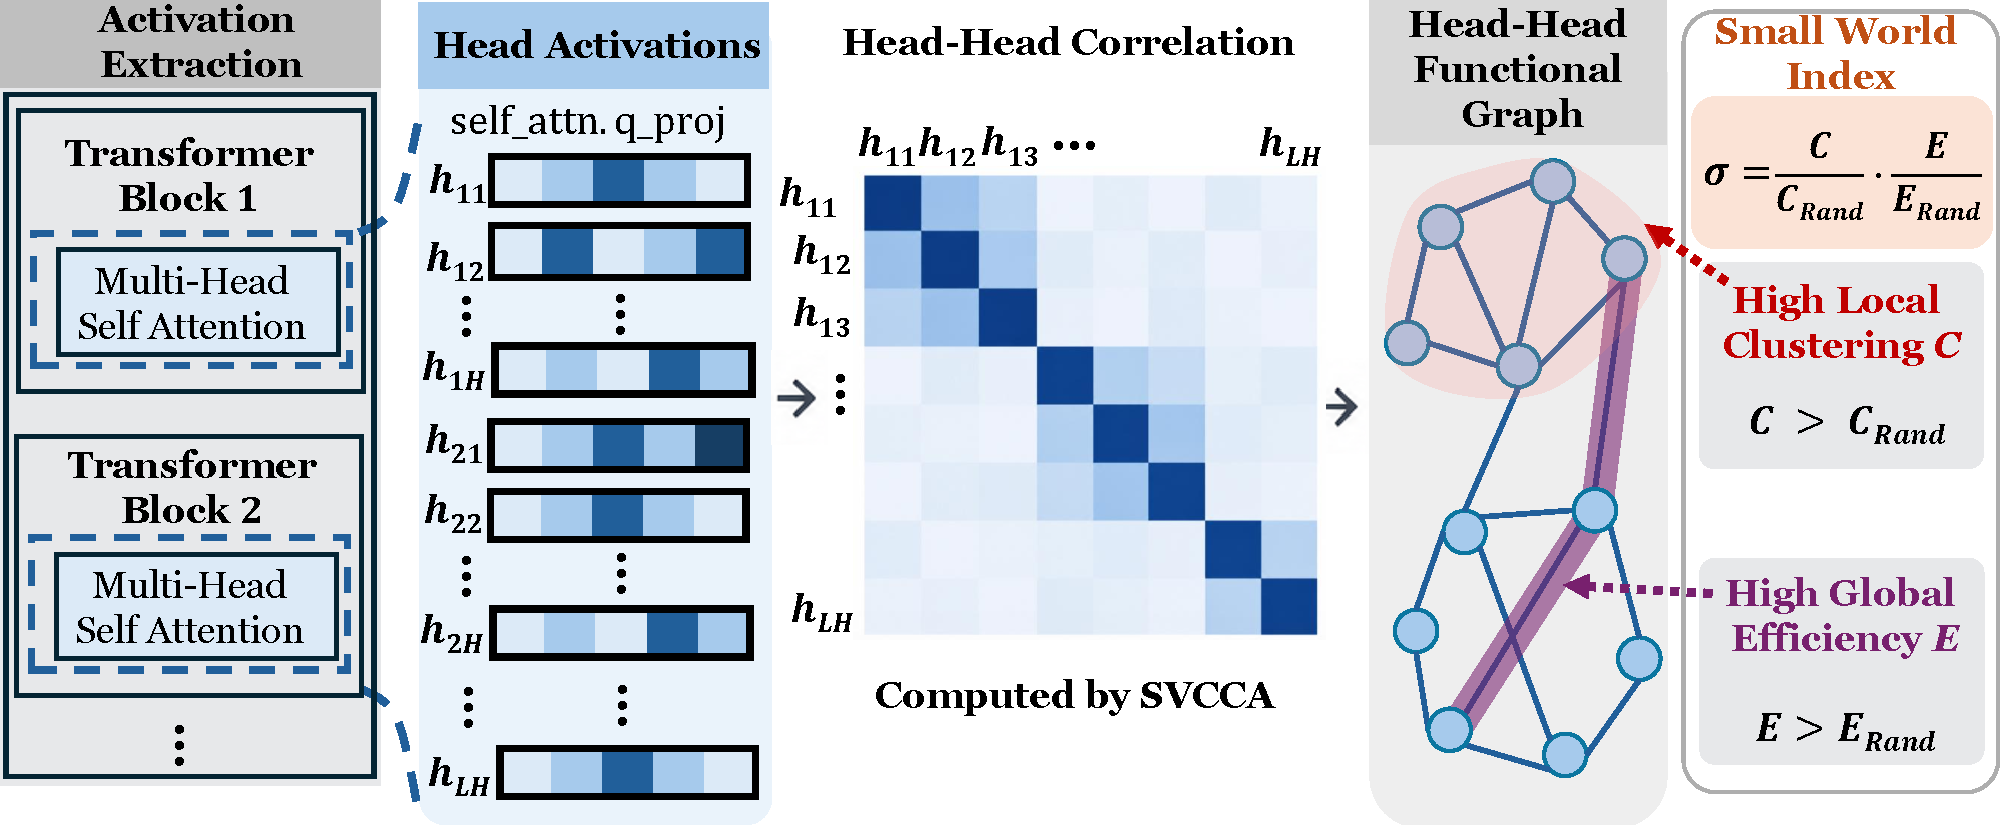
\includegraphics[width=0.85\linewidth]{figure/nips_figure_26_new.pdf}
    \caption{\small We extract activations from attention heads across Transformer layers and compute pairwise similarity (SVCCA) to construct a head-level functional graph. The resulting graph exhibits small-world structure, characterized by high clustering and efficient short-path communication. We show that this structural property correlates with model capability on fluid intelligence benchmarks.}
    \label{fig:process}
\end{figure}

In this section, we present our framework for constructing functional graphs of attention heads and quantifying their small-world organization. We first show how we construct an attention-head functional graph and compute its SWI (\Cref{sec:constructing-head}). Second, we show that SWI is associated with LLM performance on fluid intelligence benchmarks (\Cref{sec:quantify_swi}). The process is shown in~\Cref{fig:process}.



% \subsection{Constructing Functional Graphs of Attention Heads}
% \label{sec:constructing-head}
% \paragraph{Activation collection.}
% We collect attention-head activations on DRE-Bench, a dynamic benchmark for evaluating LLM fluid intelligence through abstract reasoning tasks \cite{yang2025truly}. Its tasks assess attribute-level, spatial, sequential, and conceptual reasoning, and use dynamically generated variants to test whether models can infer latent rules.\yy{the following introduction of the functional graph construction needs major revision. It should be introduced in an organized way: first introduce high level: what are the nodes and what are the edges. then give rationale by linking it to neuroscience. what analogies you are making: brain regions<->attention heads, correlation of activations<->correlation of attention acitivation. then talk a bit in detail, how do you obtain the activations and then how you compute the SVCCA similarity to obtain the edges. Also you need to provide intuition of using SVCCA. You should unlike neuroscience where ROI has scalar activation each time, each attention head produce a vector for each sample, so we need new definition for attention head similarity. This similarity should be invariant to permutation of embedding features and also need to account for the fact that attention heads from different layers may reside in different latent space. Thus, we propose to use SVCCA similarity becasue it satisifies these requirements... Then introduce SVCCA}
% Let an LLM contain $L$ transformer blocks and $H$ attention heads per block, yielding $M=L\times H$ heads in total. We sample $N$ questions from DRE-Bench, denoted as $\{x^{(n)}\}_{n=1}^{N}$. For each question $x^{(n)}$, let $T_n$ denote the number of tokens generated in its answer. We record the query activations of all self-attention heads at each generated answer token, since query activations determine which context tokens each head attends to during generation \cite{elhage2021mathematical}. This yields an activation tensor:
% \[
% \mathbf{A}^{(n)} \in \mathbb{R}^{M \times T_n \times d},
% \]
% where $d$ is the head dimension and $\mathbf{A}^{(n)}_{m,t,:}$ denotes the query activation of head $m$ at the $t$-th generated answer token. For each head and question, we average its token-level activations over the generated answer tokens:
% \[
% \mathbf{z}^{(n)}_m =
% \frac{1}{T_n}\sum_{t=1}^{T_n}\mathbf{A}^{(n)}_{m,t,:},
% \qquad
% \mathbf{z}^{(n)}_m \in \mathbb{R}^{d}.
% \]
% Stacking these vectors over all $N$ questions gives the activation matrix for head $m$:
% \[
% \mathbf{X}_m =
% \left[
% \mathbf{z}^{(1)}_m;
% \mathbf{z}^{(2)}_m;
% \dots;
% \mathbf{z}^{(N)}_m
% \right]
% \in \mathbb{R}^{N\times d}.
% \]
% Each row of $\mathbf{X}_m$ corresponds to the query activation of head $m$ for one DRE-Bench question. We use $\mathbf{X}_m$ to compute activation similarity between pairs of attention heads.






% \paragraph{SVCCA similarity.}
% Given the activation matrices $\{\mathbf{X}_m\}_{m=1}^{M}$, we compute pairwise similarity between attention heads using Singular Vector Canonical Correlation Analysis (SVCCA) \cite{raghu2017svcca}. For each pair of heads $(i,j)$, we first apply singular value decomposition (SVD) to $\mathbf{X}_i$ and $\mathbf{X}_j$ and retain the principal directions that explain a fraction $\tau$ of the variance. 
% %We use $\tau=0.99$ in our experiments. 
% We then apply canonical correlation analysis (CCA)~\cite{thompson2000canonical} to the reduced representations, obtaining canonical correlations $\{\rho_k\}_{k=1}^{r_{ij}}$, where $r_{ij}$ is the number of retained CCA dimensions.

% We define the activation similarity between heads $i$ and $j$ as the average canonical correlation:
% \[
% S_{ij}=\frac{1}{r_{ij}}\sum_{k=1}^{r_{ij}} \rho_k,
% \qquad S_{ii}=1.
% \]
% This yields a symmetric head-similarity matrix $\mathbf{S}\in[0,1]^{M\times M}$, where larger values indicate more similar activation patterns across DRE-Bench questions.
\subsection{Constructing Functional Graphs of Attention Heads}
\label{sec:constructing-head}
% we follow ns to build graph, we 类比 xxxx. we follow the way ns build graph that we xxx. 先算correlation 再算threhold then we show how we create the graph
% have the 3.2 threshold to 3.1, and 3.2 only has finding.
% 

% move svcca to prelim

% sec4 say validate. our idea is that we want to preserve SWI in pruning.

% 4.2 开头：based on the local cores we obtained, we propose. 4.2 add pruing priority scores

% layer include all modules within the block
% assign budge proportional to scores.


We first collect attention-head activations on DRE-Bench~\cite{yang2025truly}, whose tasks assess attribute-level, spatial, sequential, and conceptual reasoning. We follow the standard construction of functional brain networks: anatomical ROIs are treated as nodes, pairwise functional connectivity is estimated from statistical dependencies between their activity time series, and a graph is obtained by thresholding the resulting connectivity matrix. Analogously, we treat attention heads as nodes and estimate pairwise functional connectivity from activation-based similarity between heads. We then threshold the resulting head-similarity matrix to construct an attention-head functional graph.



% In order to build the graph of attention heads, we first collect attention-head activations on DRE-Bench \cite{yang2025truly}, which assess attribute-level, spatial, sequential, and conceptual reasoning. We then define nodes as attention heads and edges as activation-based similarities between heads. This construction is inspired by functional brain networks, where anatomical ROIs are treated as nodes and edges are estimated from statistical dependencies between their activity time series. In brain networks, functional connectivity is often estimated by Pearson correlation between scalar ROI activity time series \cite{biswal1995functional, fox2005human}. Since attention heads produce vector-valued activations, we propose use SVCCA as a multivariate analogue of correlation that measures shared correlated subspaces between heads. Detailed justification of using SVCCA is in \Cref{app:svcca_justification} of the Appendix. \yy{Since you already have a beginning paragraph in Section 3, you do not repeat again. I would suggest delete this paragraph and integrate the information to the following subsections. }

\paragraph{Activation Collection.}
% We collect attention-head activations on DRE-Bench, a dynamic benchmark for evaluating LLM fluid intelligence through abstract reasoning tasks \cite{yang2025truly}. 
% Its tasks assess attribute-level, spatial, sequential, and conceptual reasoning, and use dynamically generated variants to test whether models can infer latent rules.

Let an LLM contain $L$ transformer blocks and $H$ attention heads per block, yielding $M=L\times H$ heads in total. We sample $N$ questions from DRE-Bench \cite{yang2025truly}, denoted as $\{x^{(n)}\}_{n=1}^{N}$. For each question $x^{(n)}$, let $T_n$ denote the number of tokens generated in its answer. We record the query activations of all self-attention heads at each generated answer token.
% , since query activations determine which context tokens each head attends to during generation \cite{elhage2021mathematical}. 
This yields an activation tensor:
$
\mathbf{A}^{(n)} \in \mathbb{R}^{M \times T_n \times d},
$
where $d$ is the head dimension and $\mathbf{A}^{(n)}_{m,t,:}$ denotes the query activation of head $m$ at the $t$-th generated answer token. For each head and question, we average its token-level activations over the generated answer tokens:
$
\mathbf{z}^{(n)}_m =
\frac{1}{T_n}\sum_{t=1}^{T_n}\mathbf{A}^{(n)}_{m,t,:}, \mathbf{z}^{(n)}_m \in \mathbb{R}^{d}.
$

Stacking these vectors over all $N$ questions gives the activation matrix for head $m$:
$
\mathbf{X}_m =
\left[
\mathbf{z}^{(1)}_m;
\mathbf{z}^{(2)}_m;
\dots;
\mathbf{z}^{(N)}_m
\right]
\in \mathbb{R}^{N\times d}.
$
Each row of $\mathbf{X}_m$ corresponds to the query activation of head $m$ for one DRE-Bench question.


\paragraph{SVCCA Similarity.}
In functional brain networks, connectivity is often estimated using Pearson correlation between scalar ROI activity time series~\cite{biswal1995functional, fox2005human}. Attention heads, however, produce vector-valued activations. We therefore use SVCCA as a multivariate analogue of correlation, measuring shared correlated subspaces between heads. Additional justification for using SVCCA is provided in Section~\ref{app:swa_svcca_justification}. To compute pairwise head similarity using SVCCA as defined in~\Cref{sec:svcca_prelim}, we treat the activation matrix $\mathbf{X}_m$ of each head as its representation over DRE-Bench questions. For each pair of heads $(i,j)$, we define
$
S_{ij}=\mathrm{SVCCA}(\mathbf{X}_i,\mathbf{X}_j), S_{ii}=1.
$
This yields a symmetric head-similarity matrix $\mathbf{S}\in[0,1]^{M\times M}$, where larger values indicate more similar activation behavior across DRE-Bench questions.

\paragraph{Graph Construction.}
Following convention to construct brain graphs, we construct the graph of attention heads by thresholding the head-similarity matrix. Let $\mathcal{P}$ denote the set of all unordered pairs of distinct heads. For a target edge density $\delta$, we rank pairs in $\mathcal{P}$ by $S_{ij}$ and retain the top $K_\delta=\lfloor \delta |\mathcal{P}| \rfloor$ pairs as edges. This yields an undirected head--head functional graph
$
\mathcal{G}_\delta=(\mathcal{V},\mathcal{E}_\delta),
$
where $\mathcal{V}=\{1,\ldots,M\}$ is the set of attention heads.


\subsection{Connection of Small-world Index to Fluid Intelligence}
\label{sec:quantify_swi}
We find that \textbf{stronger small-world organization in head-head functional graphs is associated with better fluid reasoning performance} by computing the SWI of $\mathcal{G}_\delta$, following~\Cref{eq:swi}. Specifically, for each model, we compute SWI from the head-head functional graph constructed on DRE-Bench and evaluate performance using the mean per-token negative log-likelihood over the answer tokens (NLL/token), where lower values indicate better performance. As shown in Table~\ref{tab:dre_perf_swi_levels}, models with lower NLL consistently exhibit higher SWI. Qwen3-14B achieves the strongest performance and the highest SWI, while Llama-3.2-1B has the weakest performance and the lowest SWI. The trend remains consistent across models, suggesting that stronger small-world functional organization is associated with better fluid reasoning performance. The setup details are in \Cref{sec:swa_exp_setup}.

\begin{table}[t]
\centering
\small
\setlength{\tabcolsep}{4pt}

\caption{\small Relationship between DRE-Bench performance and small-world organization.
We report the mean per-token negative log-likelihood over the answer tokens (NLL/token; lower is better) and SWI of the head-head functional graph on DRE-Bench Level 1 and Level 2 tasks. Results are averaged over three seeds and reported as mean$_{\pm \text{std}}$. Across models, lower NLL is associated with higher SWI.}

\begin{tabular}{lcccc}
\toprule
\textbf{Model} 
& \multicolumn{2}{c}{\textbf{Level 1}} 
& \multicolumn{2}{c}{\textbf{Level 2}} \\
\cmidrule(lr){2-3} \cmidrule(lr){4-5}
& \textbf{NLL/token} $\downarrow$
& \textbf{SWI} $\uparrow$
& \textbf{NLL/token} $\downarrow$
& \textbf{SWI} $\uparrow$ \\
\midrule
Qwen3 14B 
& 0.0822$_{\scriptstyle \pm 0.01}$ & 1.8160$_{\scriptstyle \pm 0.27}$
& 0.2410$_{\scriptstyle \pm 0.03}$ & 1.7020$_{\scriptstyle \pm 0.12}$ \\
Qwen3 8B 
& 0.0949$_{\scriptstyle \pm 0.01}$ & 1.5850$_{\scriptstyle \pm 0.28}$
& 0.2814$_{\scriptstyle \pm 0.02}$ & 1.6000$_{\scriptstyle \pm 0.07}$\\
Llama3 8B 
& 0.0980$_{\scriptstyle \pm 0.01}$ & 1.3750$_{\scriptstyle \pm 0.19}$
& 0.2993$_{\scriptstyle \pm 0.02}$ & 1.5935$_{\scriptstyle \pm 0.11}$ \\
Qwen3 4B 
& 0.1142$_{\scriptstyle \pm 0.02}$ & 1.2180$_{\scriptstyle \pm 0.26}$
& 0.3397$_{\scriptstyle \pm 0.05}$ & 1.2722$_{\scriptstyle \pm 0.18}$ \\
Llama3.2 3B 
& 0.1377$_{\scriptstyle \pm 0.07}$ & 1.1933$_{\scriptstyle \pm 0.33}$
& 0.3412$_{\scriptstyle \pm 0.10}$ & 1.2100$_{\scriptstyle \pm 0.17}$ \\
Llama3.2 1B 
& 0.1689$_{\scriptstyle \pm 0.20}$ & 0.9188$_{\scriptstyle \pm 0.49}$
& 0.5800$_{\scriptstyle \pm 0.26}$ & 0.9344$_{\scriptstyle \pm 0.18}$ \\
\bottomrule
\end{tabular}
\vspace{-0.5cm}

\label{tab:dre_perf_swi_levels}
\end{table}



% sec4 say validate. our idea is that we want to preserve SWI in pruning.

% 4.2 开头：based on the local cores we obtained, we propose. 4.2 add pruing priority scores

% layer include all modules within the block
% assign budge proportional to scores.
\section{Applying Our Finding to LLM Pruning}
\label{sec:core-bridge}
In this section, we validate the finding in~\Cref{sec:quantify_swi} by testing whether preserving small-world organization helps maintain model performance under pruning. Since SWI is a graph-level metric, while pruning decisions are typically made at finer granularity such as heads and layers, we translate global small-world organization into local measures. Specifically, we define two node-level scores corresponding to the defining properties of small-world organization: local clustering and global communication. We then use these scores to guide sparsity allocation for LLM pruning.


% \yy{Some connecting sentences that transit from the key finding to this section, e.g., From Section 3, we show that maintaining a high SWI is the key to preserve fluid intelligence of LLMs. In this section, we will show how we can apply this finding in LLM pruning. As SWI is a global metric and pruning often takes place at finer granularity, i.e., at the head and layer level. Thus, in this section, we first translate the global SWI into local measures by defining two node-level structural scores that directly capture its defining properties. We then show how we can use these scores to ...}
% In this section, we derive local structural scores from the small-world functional graph, assigning structural roles to individual heads and layers. We then use these scores to guide downstream applications such as pruning.

\subsection{Node-level Small-world Metrics}
Given $\mathcal{G}_\delta$, we define two head-level scores based on the two defining properties of small-world organization. The core score measures within-community connectivity and corresponds to local clustering, while the bridge score measures cross-community connectivity and corresponds to efficient global communication. We apply Louvain community detection~\cite{blondel2008fast} to $\mathcal{G}_\delta$ to obtain communities $\mathcal{C}_\delta=\{C_1,\ldots,C_K\}$, and let $C(i)$ denote the community containing head $i$.
\paragraph{Core Score.}

Let $C(i)$ denote the community containing head $i$, and set $S_{ij}=0$ for non-edge pairs in $\mathcal{G}_\delta$. We define the core score of head $i$ as
$
\mathrm{Core}_i =
\frac{\sum_{j\in C(i)} S_{ij}}
{\sum_{j\in \mathcal{V}} S_{ij} +\varepsilon},
$
where $\varepsilon$ is a small constant that prevents division by zero. A larger $\mathrm{Core}_i$ indicates that a larger fraction of head $i$'s total connection strength lies within its own community, suggesting that the head plays a stronger role in maintaining local community structure.
\paragraph{Bridge Score.}
For head $i$, let
$
s_{i,k}=\sum_{j\in C_k} S_{ij}
\quad\text{and}\quad
s_i=\sum_{j\in\mathcal{V}} S_{ij}.
$
We can then define
$
\mathrm{Bridge}_i
=
1-
\sum_{k=1}^{K}
\left(
\frac{s_{i,k}}{s_i+\varepsilon}
\right)^2.
$
A larger $\mathrm{Bridge}_i$ indicates that head $i$ more strongly links multiple communities \cite{pedersen2017spontaneous}.
Together, core and bridge scores characterize how individual attention heads contribute to the functional graph: core scores capture within-community connectivity, while bridge scores capture cross-community connectivity. We use these scores to guide LLM pruning.


\subsection{Pruning Method Based on Node-Level Small-World Metrics}
\label{sec:pruning}

Based on the local scores we obtained, we propose Small-World Allocation (SWA), a hierarchical sparsity allocation method that uses local small-world scores to guide pruning. The key idea is to preserve components that play important roles in the functional graph. 
SWA defines pruning priority scores at both the head and layer levels: head-level scores determine the pruning ratio for each attention head, while layer-level scores allocate sparsity across Transformer blocks. This two-level design allows SWA to balance local head importance with global layer-wise sparsity allocation.
% SWA therefore defines pruning priority scores at both the head and layer levels: head-level scores determine the pruning ratio for each attention head within a layer, while layer-level scores decide how much sparsity should be assigned to each Transformer block. This two-level design allows SWA to coordinate local head importance with global layer-wise sparsity allocation.

At the head level, we combine core and bridge scores into a pruning priority score. For each head $i$, we first convert its bridge and core scores into percentile ranks over all heads, denoted by $\tilde{B}_i \in [0,1]$ and $\tilde{C}_i \in [0,1]$, where larger values indicate stronger structural roles. We define the priority score as
\begin{equation}
p_i = (1-\tilde{B}_i)(1-\tilde{C}_i).
\end{equation}

A smaller pruning priority score $p_i$ indicates that head $i$ has a strong core or bridge role and should be preserved, while a larger $p_i$ indicates higher pruning priority. At the layer level, we aggregate head-level pruning priority scores within each layer. Let $\mathcal{H}_\ell$ denote the set of heads in layer $\ell$
\begin{equation}
p_\ell =
\frac{1}{|\mathcal{H}_\ell|}
\sum_{i\in \mathcal{H}_\ell}
p_i .
\end{equation}

A smaller score $p_\ell$ indicates that layer $\ell$ contains more structurally important heads and should receive a lower sparsity budget, while a larger $p_\ell$ indicates higher layer-level pruning priority.

SWA assigns pruning budgets in proportion to the priority scores through a hierarchical allocation procedure. Layer-level scores first determine the sparsity budget for each Transformer block, including all modules within the block; head-level scores then distribute the attention sparsity across individual heads. Following~\cite{hu2025eigenspectrum}, we normalize the scores, convert them into relative pruning ratios, and rescale the ratios so that the overall sparsity matches the target global sparsity.
